\documentclass[10pt]{article}

\usepackage[margin=0.75in]{geometry}
\usepackage{amsmath,amsthm,amssymb}
\usepackage{xcolor}
\usepackage{cancel}
\usepackage{graphicx}
\usepackage{changepage}
\usepackage{circuitikz}
\usepackage{pgfplots}
\usepackage{physics}
\usepackage{hyperref}
\usepackage{siunitx}
\usepackage{fontspec}
\usepackage{relsize}
\usepackage{subfig}
\usepackage{todonotes}
\usepackage{multicol, multirow, booktabs}
\usepackage[breakable]{tcolorbox}
\usepackage[inline]{enumitem}

\theoremstyle{definition}
\newtheorem{problem}{Problem}
\newtheorem{soln}{Solution}

\pgfplotsset{compat=newest}
\usetikzlibrary{lindenmayersystems}
\usetikzlibrary{arrows}
\usetikzlibrary{calc}
\usetikzlibrary{positioning, fit}
\usetikzlibrary{3d, perspective}

\definecolor{incolor}{HTML}{303F9F}
\definecolor{outcolor}{HTML}{D84315}
\definecolor{cellborder}{HTML}{CFCFCF}
\definecolor{cellbackground}{HTML}{F7F7F7}
\newcommand{\ui}{\hat{i}}
\newcommand{\uj}{\hat{j}}
\newcommand{\uk}{\hat{k}}
\newcommand{\ux}{\hat{x}}
\newcommand{\uy}{\hat{y}}
\newcommand{\uz}{\hat{z}}
\newcommand{\primed}[1]{#1^\prime}
\pgfdeclarelayer{background}  
\pgfsetlayers{background,main}
\AtBeginDocument{\RenewCommandCopy\qty\SI}

\makeatletter
\newcommand{\boxspacing}{\kern\kvtcb@left@rule\kern\kvtcb@boxsep}
\makeatother
\newcommand{\prompt}[4]{
    \ttfamily\llap{{\color{#2}[#3]:\hspace{3pt}#4}}\vspace{-\baselineskip}
}

\newcommand{\thevenin}[2]{
  \begin{center}
    \begin{circuitikz} \draw
      (0,0) -- (2,0) to[battery1, l_=$V_{Th}\eq#1$] (2,2) 
      to[resistor, l_=$R_{Th}\eq#2$] (0,2)
      ;
      \draw [o-] (-.07,2.079);
      \draw [o-] (-.07,0.079);
    \end{circuitikz}
  \end{center}
}

\newcommand{\norton}[2]{
  \begin{center}
    \begin{circuitikz} \draw
      (0,0) -- (3,0) to[american current source, l_=$I_{N}\eq#1$] (3,2) -- (0,2) (2,0)
      to[resistor, l=$R_{N}\eq#2$] (2,2)
      ;
      \draw [o-] (-.07,2.079);
      \draw [o-] (-.07,0.079);
    \end{circuitikz}
  \end{center}
}

\newcommand{\highlight}[1]{\colorbox{yellow}{$\displaystyle #1$}}

\newcommand{\ti}[1]{\widetilde{#1}}

\newfontface{\Kaufmann}{Kaufmann}
\DeclareTextFontCommand{\kf}{\Kaufmann}
\newcommand{\scriptr}{\fontsize{12pt}{12pt}\kf{r}}

\newfontface{\KaufmannB}{Kaufmann Bd BT}
\DeclareTextFontCommand{\kfb}{\KaufmannB}
\newcommand{\bscriptr}{\fontsize{12pt}{12pt}\kfb{r}}

\newcommand{\bv}[1]{\mathbf{#1}}

\title{Physics 3610H: Assignment II}
\author{Jeremy Favro (0805980) \\ Trent University, Peterborough, ON, Canada}
\date{\today}

\begin{document}
\maketitle

% PROBLEM 1
\begin{problem} Consider a single particle of mass m moving in one dimension subject to the following
potential:
$$
  V(x)=\begin{cases}
    \infty, & x<-c   \\
    0,      & -c<x<c \\
    \infty, & x>c
  \end{cases}
$$
\begin{enumerate}[label=(\alph*)]
  \item Find the eigenvalues and eigenstates of $\hat{H}$ for this system, that is the energies $E$ and the
        states $\psi$ for which $\hat{H}\psi=E\psi$.
  \item Examine the two lowest energy states:
        \begin{enumerate}[label=(\roman*)]
          \item Draw two plots showing $\psi$ vs $x$ for the two lowest energy states.
          \item This is very similar to the problem we solved in class. Comment on whether your results
                for the two lowest energy states (both the energies and the states) are consistent with those
                we found in class.
          \item Show that the two lowest energy states are orthogonal.
        \end{enumerate}
\end{enumerate}
\end{problem}
\begin{soln}~
  \begin{enumerate}[label=(\alph*)]
    \item Here $\hat{H}$ is the operator corresponding to the total energy of the particle. Because the particle is only subject to the potential
          applied by the well at its edges and possesses only kinetic energy otherwise we can say
          $$\hat{H}=-\frac{\hbar^2}{2m}\frac{\partial}{\partial x} + V(x)$$
          where we've obtained the operator corresponding to kinetic energy by using the momentum operator in the usual expression for kinetic energy.
          Now that we have $\hat{H}$ we can solve the time dependent Schr\"odinger equation,
          $$i\hbar\frac{\partial}{\partial t}\Psi(x,t)=\hat{H}\Psi(x,t)$$
          which, when we substitute our $\hat{H}$ becomes
          $$i\hbar\frac{\partial}{\partial t}\Psi(x,t)=\left[-\frac{\hbar^2}{2m}\frac{\partial^2}{\partial x^2} + V(x)\right]\Psi(x,t).$$
          We will try now to find a $\Psi(x,t)$ which is separable as $\Psi(x,t)=\psi(x)\phi(t)$ this doesn't always work but from some foreknowledge
          of the problem we know there is a fair chance that it will and so we try it. This means that our equation is now
          $$i\hbar\frac{\partial}{\partial t}\psi(x)\phi(t)=\left[-\frac{\hbar^2}{2m}\frac{\partial^2}{\partial x^2}  + V(x)\right]\psi(x)\phi(t).$$
          We can divide through on both sides by $\psi(x)\phi(t)$ being careful to note that we cannot pull functions out of derivatives that contain
          the variable of differentiation, e.g. on the left side $\phi$ will not cancel and the derivative will instead be multiplied out front
          by $\phi^{-1}$. This makes our equation now
          $$\frac{i\hbar}{\phi(t)}\frac{\partial}{\partial t}\phi(t)=\frac{1}{\psi(x)}\left[-\frac{\hbar^2}{2m}\frac{\partial^2}{\partial x^2}  + V(x)\right]\psi(x)$$
          which satisfies our original reason for trying to separate $\Psi$: to obtain two differential equations of only on variable each which makes them ODEs instead
          of PDEs. Another consequence of this separation while maintaining equality is that these functions must \emph{always} be equal. The only way this can happen
          is if both are equal to a constant as fixing one variable and varying the other would (if they were not equal to a constant), to preserve equality, require that $x$ and $t$
          are related in a way that makes this possible. This is obviously not the case so we can reason that regardless of values of $x$ or $t$, the two must be the same and constant.
          This allows us to further ``separate'' the equation into two independent ODEs,
          \begin{align}
            E & =\frac{i\hbar}{\phi(t)}\frac{d}{d t}\phi(t) \label{eq1}                                      \\
            E & =\frac{1}{\psi(x)}\left[-\frac{\hbar^2}{2m}\frac{d^2}{d x^2} + V(x)\right]\psi(x)\label{eq2}
          \end{align}
          We will first begin by solving \ref{eq1} as it is very easy by recognizing that there is an easy function who's derivative is itself times a constant, $e^x$.
          This gives us
          $$\phi=Ce^{-iEt/\hbar}$$
          where $A$ is a constant of integration that we will determine later.
          Now for \ref{eq2} with some rearranging (and noticing the $V(x)=0$ in the region we care about) we have
          $$-\frac{2mE}{\hbar^2}\psi(x)=\frac{d^2}{d x^2}\psi(x).$$
          This means we are looking now for a function whose second derivative is itself times a negative constant. \todo{Why choose sin}
          Using the theorem given that functions for such a system must be either even or odd I choose to use an even function which also satisfies the derivative
          property above, $\sin x$. We must however be careful to note that however we set up our $\psi(x)$ it must obey the physical constraint that
          the particle cannot be found at $-c$ as it would need sufficient energy to pass a potential barrier of infinite energy which is impossible. We can use this knowledge to say that
          $$\psi(x)=\sin\left(k(x+c)\right)$$
          where $k=\sqrt{\frac{2mE}{\hbar^2}}$. This, at $-c$, becomes $\sin (0)=0$. Now we must consider the upper bound of the well where we enforce the same constraint for the same reasons,
          $$ \psi(c) =0= A\sin\left(2kc\right)=A\sin\left(2\sqrt{\frac{2mE}{\hbar^2}}c\right) $$
          This gives us two constants to mess with to satisfy the equality, $A$ and $E$. To make this zero using $A$ would require $A=0$ which is a trivial solution which gives us no information
          and says that the particle does not exist. We instead choose to determine an $E$ such that the equation is zero. Given that $\sin(x)$ is zero for all
          $x=2n\pi$ where $n\in \mathbb{Z}$ we need to find an $E$ that gives this. However we must first trim our bound on $n$ down a bit as $n=0$ gives us
          again the no-particle solution over the entire well and not just the edges as we want here
          and the negative $n$s result in only a change in $A$ as $\sin(-x)=\sin(x)$ meaning they are linearly dependent and therefore superfluous in combination with the
          positive solutions. We therefore adopt the final form of $\psi(x)$,
          $$\psi(x)=A\sin\left(2\sqrt{\frac{2E_nm}{\hbar^2}}x\right)$$
          where $E_n=\displaystyle\frac{\hbar^2n^2\pi^2}{8mc^2}$ where $n\in \mathbb{Z}^{>0}$ (integers $1,2,3,\dots$).
          To find $A$ we use the condition that the probability of the particle existing (being found anywhere) must be $1$. This means that
          $$\int_{-\infty}^{\infty}\left|\Psi(x,t)\right|^2dx=1.$$
          We can simplify this a bit by noting that the time dependent part of $\Psi$ cancels itself out when multiplied with its conjugate
          as we are doing in the integral and also noting that, as mentioned earlier, the particle may only exist in the well so the bounds can
          be reduced to $-c\to c$,
          \begin{align*}
            1 & =\int_{-c}^{c}\psi(x)\psi^*(x)dx                                                                                         \\
              & =\int_{-c}^{c}\left|A\right|\sin\left(\frac{n\pi}{c}x\right)\left|A\right|\sin\left(\frac{n\pi}{c}x\right)dx             \\
              & =\left|A\right|^2\int_{-c}^{c}\sin^2\left(\frac{n\pi}{c}x\right)dx                                                       \\
              & =\left|A\right|^2\int_{-c}^{c}\frac{1-\cos\left(2\frac{n\pi}{c}x\right)}{2}dx                                            \\
              & =\left|A\right|^2\left(\int_{-c}^{c}\frac{1}{2}dx-\int_{-c}^{c}\frac{\cos\left(2\frac{n\pi}{c}x\right)}{2}dx\right)      \\
              & =\frac{\left|A\right|^2}{2}\left(2c-\cancel{\frac{c}{2n\pi}\left[\sin\left(2\frac{n\pi}{c}x\right)\right]_{-c}^c}\right) \\
              & 1=c\left|A\right|^2\implies \left|A\right|=\sqrt{\frac{1}{c}}\implies A=\sqrt{1/c}
          \end{align*}
          So we have
          $$\psi(x)=\sqrt{1/c}\sin\left(\frac{n\pi}{c}x\right).$$
          Which gives us our eigenfunctions $\psi_n(x)$ and our eigenvalues
          $$E_n=\displaystyle\frac{\hbar^2n^2\pi^2}{8mc^2}.$$
          \newpage
    \item ~\\
          \begin{enumerate}[label=(\roman*)]
            \item ~\\ \begin{center}
                    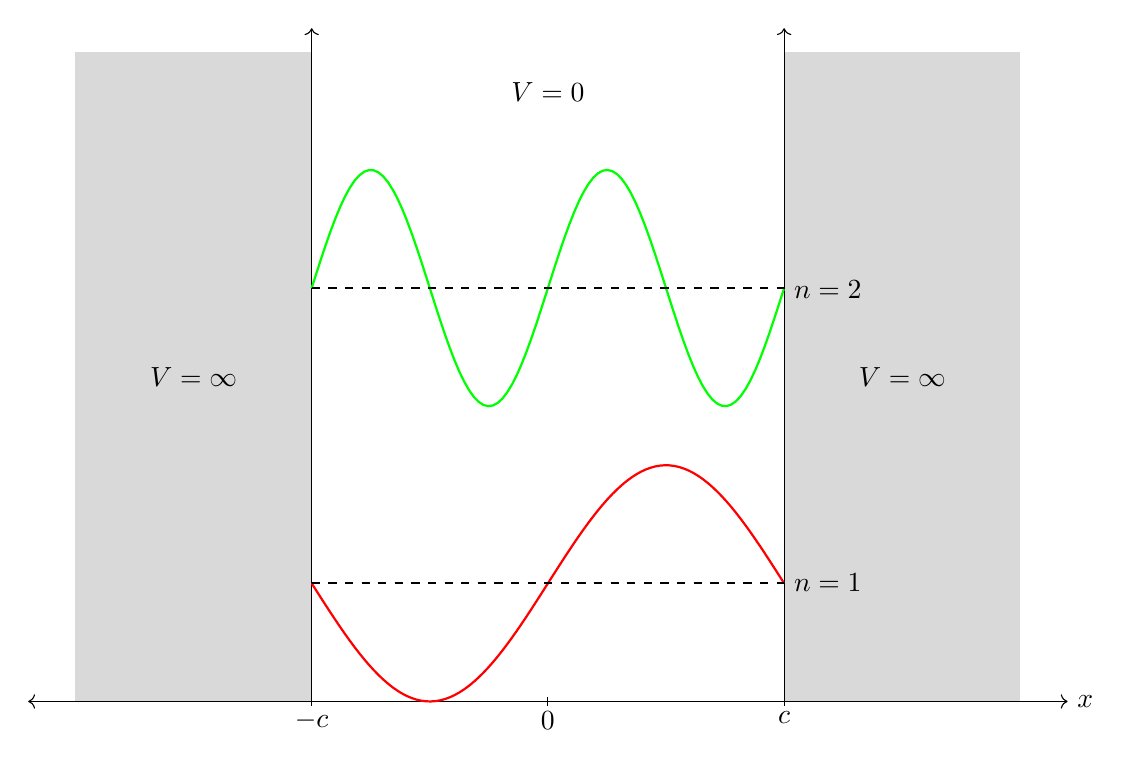
\begin{tikzpicture}[x=2cm, scale=1.5]
                      \def\topval{5.5}
                      \fill[gray!30]
                      (-1, 0) rectangle (-2, \topval);
                      \fill[gray!30]
                      (1, 0) rectangle (2, \topval);
                      \node at (-1.5, \topval/2) { $V = \infty$};
                      \node at (1.5, \topval/2) {$V = \infty$};

                      \node[anchor = north] at (-1, 0)   { $-c$};
                      \node[anchor = north] at (0, 0)   {0};
                      \node[anchor = north] at (1, 0)   {$c$};
                      \node[anchor = west] at (2.2, 0)   {$x$};
                      \node[anchor = south] at (0, \topval-0.5) { $V = 0$};
                      \draw[<->] (-2.2, 0) to (2.2, 0);
                      \draw[] (0,-0.04) -- (0,0.04);
                      \draw[->]  (1, -0.04) to (1, \topval+0.2);
                      \draw[->]  (-1, -0.04) to (-1, \topval+0.2);


                      %Functions

                      \draw[red, thick, domain=-1:1, samples=100] plot (\x, {sin(deg(pi*\x))+1}) node[right, black] {$n=1$};
                      \draw[dashed, thick] (-1,1) --(1,1);
                      \draw[green, thick, domain=-1:1, samples=100] plot (\x, {sin(deg(2*pi*\x))+3.5}) node[right, black] {$n=2$};
                      \draw[dashed, thick] (-1,3.5) --(1,3.5);
                      % \draw[blue, thick, domain=0:4, samples=200] plot (\x, {sin(360*\x/4)}) ;
                      % \draw[green, thick, domain=0:4, samples=200] plot (\x, {sin(540*\x/4)})  ;
                    \end{tikzpicture}
                  \end{center}
            \item In the example in class we solved for a well with width $a$ (running from $0\to a$). Our energy here for $n=1$ is
                  $$E_1=\frac{\hbar^2\pi^2}{8mc^2}$$

            \item Orthogonality on functions is defined using the inner product of functions,
                  $$\int_{-c}^c f(x)g(x)\,dx$$
                  with the typical definition of orthogonality (0 means orthogonal). So,
                  \begin{align*}
                     & =\int_{-c}^c\psi_1(x)\psi_2(x)\,dx                                                                                          \\
                     & =\int_{-c}^c\sqrt{1/c}\sin\left(\frac{\pi}{c}x\right)\sqrt{1/c}\sin\left(\frac{2\pi}{c}x\right)\,dx                         \\
                     & =\frac{1}{c}\int_{-c}^c\sin\left(\frac{\pi}{c}x\right)\sin\left(\frac{2\pi}{c}x\right)\,dx                                  \\
                     & =\frac{1}{2c}\int_{-c}^c\cos\left(\frac{\pi}{c}x-\frac{2\pi}{c}x\right)-\cos\left(\frac{\pi}{c}x+\frac{2\pi}{c}x\right)\,dx \\
                     & =\frac{1}{2c}\int_{-c}^c\cos\left(-\frac{\pi}{c}x\right)-\cos\left(\frac{3\pi}{c}x\right)\,dx                               \\
                     & =-\frac{c}{6c\pi}\left[\sin\left(\frac{3\pi}{c}x\right)-3\sin\left(\frac{\pi}{c}x\right)\right]_{-c}^c=0
                  \end{align*}
          \end{enumerate}
  \end{enumerate}
\end{soln}
\end{document}